\section*{Design}\label{design}

% System Architecture (Your idea)
% • Prototyping (how you implemented it)
% • Testing (how you are going to test it → Result)

\subsection{Architecture}\label{architecture}

\begin{figure}[h]
  \begin{center}
    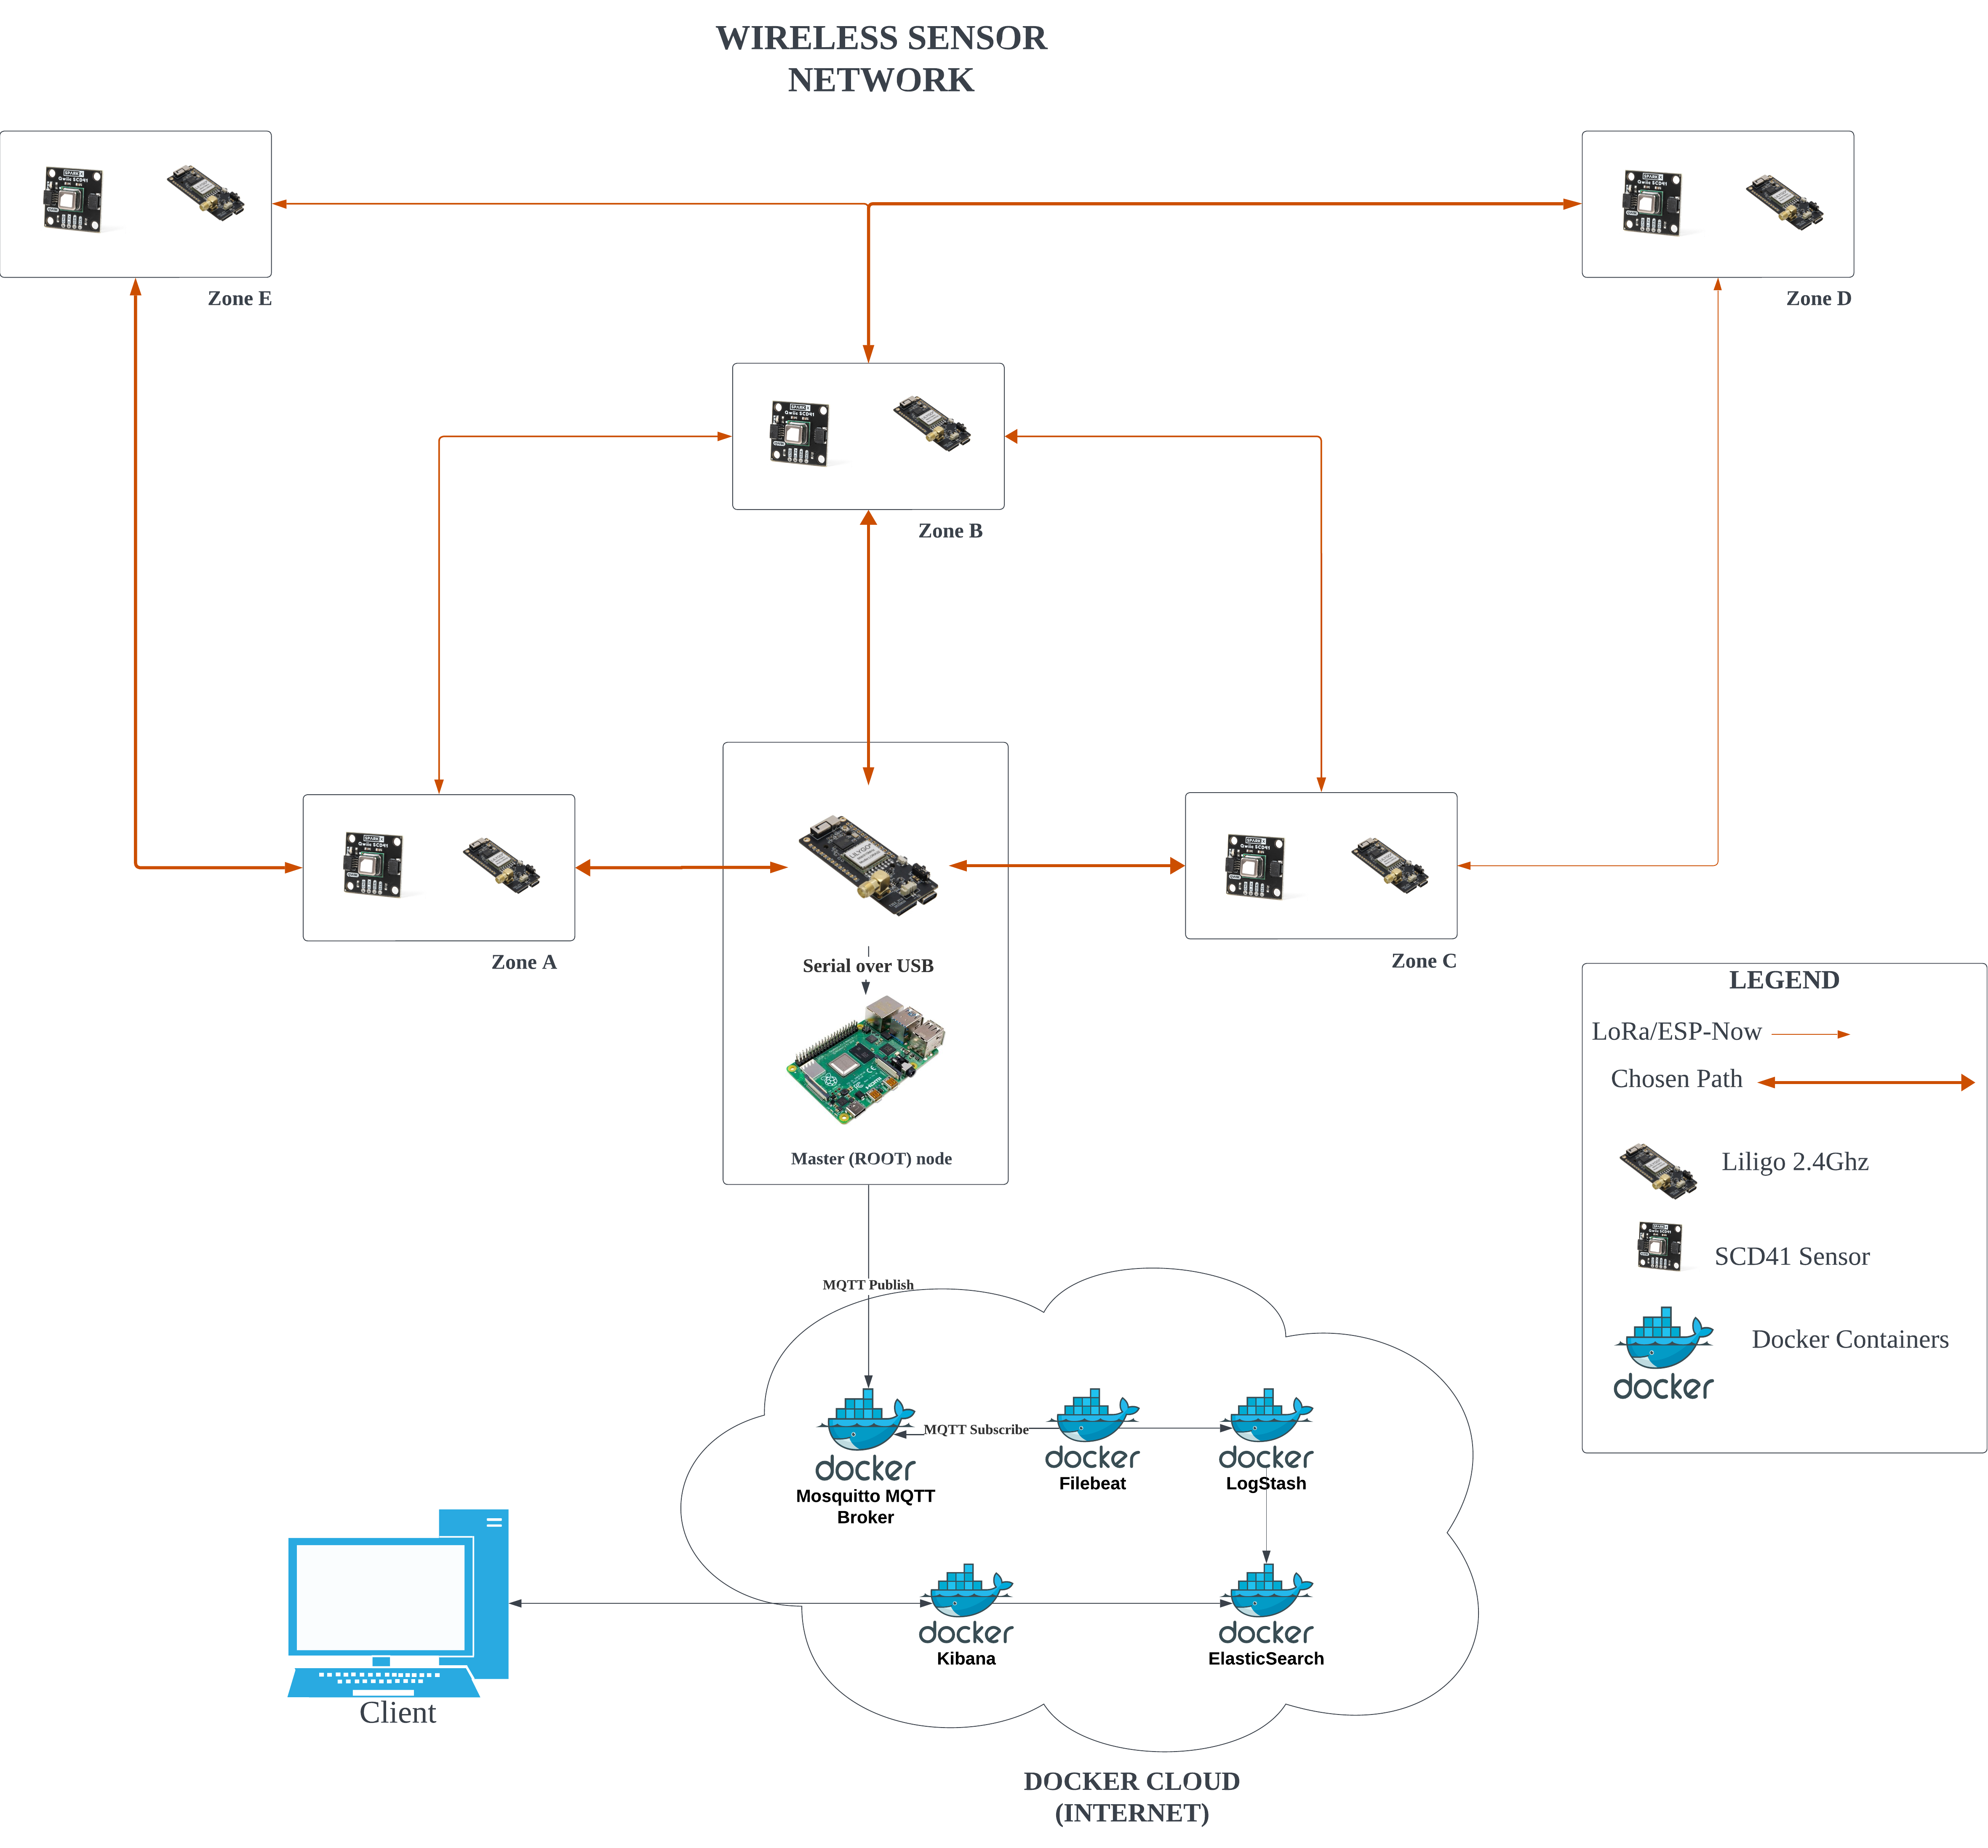
\includegraphics[width=0.35\textwidth]{./Figures/architecture.png}
  \end{center}
  \caption{Proposed System Architecture}\label{architecture}
\end{figure}

Our system architecture aims to streamline data collection and analysis from a Wireless Sensor Network (WSN) Mesh, comprising two main components: the WSN Mesh itself and the data collection sink. Sensor nodes equipped with the Liligo T3S3 Lora 2.4Ghz module form the WSN Mesh, communicating via ESP-Now and LoRa Protocols for efficient node discovery and routing. The root node establishes a MQTT connection with the broker via a Raspberry Pi 4b, responsible for aggregating data from the WSN Mesh and forwarding it to the Elasticsearch, Logstash, and Kibana Stack (ELK Stack) for visualization and analysis.

\subsection{Prototyping}\label{prototyping}
For prototyping, our strategy involves deploying sensor nodes equipped with the Liligo T3S3 Lora 2.4Ghz module. These nodes will utilize ESP-Now and LoRa Protocols for seamless communication. One node will be connected to the SCD41 Sensor, while others will generate synthetic data. The root node will establish a connection to the sink via MQTT, ensuring smooth data collection, analysis, and visualization. As an enhancement, we aim to implement protocol switching to adapt to fluctuating network conditions.

% Modified 10/3/24%
We intend to develop a modified algorithm (\textbf{DSR}) for each protocol. Each protocol mesh will include a common master node, configured with Message Queueing Technology (MQTT). This master node will interface with the backbone ELK Stack through Mosquitto MQTT Broker and filebeat with Elasticsearch for data aggregation. Kibana will be used for visualization.

% We intend to utilize two libraries (\textbf{espNowFloodingMeshLibrary,}) for each of the protocols. Additionally, we will develop a modified algorithm (\textbf{DSR}) for each protocol. Each protocol mesh will include a common master node, configured with Message Queueing Technology (MQTT). This master node will interface with the backbone ELK Stack through Mosquitto MQTT Broker and filebeat with Elasticsearch for data aggregation. Kibana will be used for visualization.


\subsubsection{ESP-Now Prototype}
% Jovian/Ben doing this, don touch %


% ESP NOW implementation draft 1.0 by Jovian %
% Benben korkor help read and modify accordingly pl0x <3 %
In crafting a sophisticated network for environmental monitoring, our collective effort harnessed the combined strengths of the ESP-NOW protocol and the Dynamic Source Routing (DSR) algorithm. This integrated approach was strategically chosen to navigate the intricate challenges associated with collecting and analyzing environmental data in real time. Engineered to deliver exceptional efficiency, flexibility, and scalability, the network stands poised to fulfill the stringent demands of a wide array of environmental monitoring projects.

The initial phase involved setting up ESP32 modules to operate with ESP-NOW, a protocol distinguished by its minimal power usage and effective direct communication features. This choice was motivated by the need for a system capable of operating in energy-constrained environments while maintaining reliable data transmission over short distances. The integration of environmental sensors, such as those for measuring temperature, humidity, and air quality, was a critical step in enabling the network to collect a wide range of data, vital for comprehensive environmental analysis.

To enhance the network's adaptability and efficiency in data routing, we will develop a custom implementation of the Dynamic Source Routing (DSR) algorithm across the devices. DSR's flexible, on-demand routing mechanism will allow the network to dynamically adjust to changes and maintain data flow when required, even in the face of node failures or alterations in network topology. This will ensure uninterrupted collection and transmission of environmental data, a key requirement for real-time monitoring applications.

% i rephrased slightly to this benben, future tense oni %
In our planned setup using ESP-NOW, each peer node will regularly collect data from its SCD41 sensor. It will then consult its peer list, which will serve as a routing table, containing only the MAC addresses of the root node and those peer nodes that are either directly linked to the root node or have knowledge of the route to it. The node will then send the data from the SCD41 sensor to an appropriate node available in its peer list.

% i rephrased slightly to this benben, future tense oni %
Should the peer list be empty, indicating there are no known routes, the node will initiate a route discovery process by sending out a broadcast request to surrounding nodes. When a node receives such a request, it will respond if it knows the way to the root node. The node that made the request will update its peer list with this new route information from any responder. This route discovery will continue until all neighbouring nodes have been discovered. We will also implement a hop count list to refine routing efficiency, allowing the peer node to choose the route with the shortest path to the root node to ensure the most efficient data transmission within our routing framework.

Another pivotal component of our system will be the central ESP32 module, designated as the master node. This module will serve a dual purpose: it will act as a receiver for data collected via ESP-NOW from the sensor-equipped nodes and as a transmitter, forwarding this data to a cloud service or server via WiFi using the MQTT protocol. This dual functionality will enable seamless integration of the sensor network with internet-based data processing and analysis tools, extending the capabilities of our monitoring system beyond local data collection.

% Not needed
% On the server side, the use of an MQTT broker facilitates efficient reception and handling of the data transmitted by the master node. Subsequently, the data is aggregated and stored using Elasticsearch, which provides a robust platform for data indexing and search capabilities. To make the data actionable, we utilized Kibana for real-time visualization, enabling the creation of dynamic dashboards that display environmental data trends, patterns, and anomalies. This comprehensive approach to data management and analysis allows for in-depth understanding and informed decision-making based on the collected environmental data.


\subsubsection{LoRa Prototype}

In our planned deployment of a LoRa mesh network, distinct from our ESP-NOW prototype, we aim to construct a network architecture that features a central node equipped with internet capabilities and several leaf nodes to establish the mesh. Every node within this architecture will be assigned a distinct identifier, possibly through methods like UUID, to assure uniqueness throughout the network. The central node will facilitate network coordination and internet-based data transmission, while the leaf nodes will focus on tasks such as sensing and data gathering.

% Upon joining the network, a new leaf node will initiate its integration by broadcasting a "route discovery message" (RDM) and then waiting for replies. This RDM will be specifically structured to include a message type indicator, the sender's ID, and a list starting with the sender's ID essential for routing. As the message moves through the network, nodes receiving it will check the list. If they are not already listed, they will add their ID and pass the message on, ensuring it eventually reaches the central node and maps out the most direct routes.

Upon starting up the master nodes and leaf nodes for setup, the master node will start listening for a "route discovery message" (RDM). This RDM will be structured to contain a message type, the node's level (indicates number of hops from master node) and the node's MAC address as a unique identifier. The leaf nodes broacast its RDM to its neighbouring nodes. When a node receives a RDM, it saves the nodes with the lowest level in the node. 

% After the central node receives the RDM, it will alter the message to a "route discovery reply message" (RDRM) and send it back. Nodes in receipt of this message will verify if their ID is at the end of the list; if so, they'll reorder their ID to the beginning before rebroadcasting. If their ID isn't at the end, the message is disregarded. The node that initiated the route discovery will store the paths in its "routing table" (RT), lining up multiple potential routes.

After saving the the Address and level of the peer node RDM a leaf node has received, the node raises its node level by one, indicating that it is one level higher further from the master node from a known route to the master node. The node then broadcast its RDM to its surrounding nodes. Nodes will ignore messages with a level higher than iteself. This process will continue until the timer ends and all niehgbouring peer routes have been stored in each node's "routing table" (RT), lining up multiple potential routes.

% For transmitting data, a leaf node will pick the primary route in its RT, tag this onto a "data message" (DM) along with its ID and a data indicator, and then wait for a "data reply message" (DRM) from the central node. Should a DRM not be received within a certain period, the node will try resending the DM via a different route from its RT, making use of various RDRMs to find another viable path.

For data transmission, the leaf node will pick the first route saved in its routing table and now send the message packet to that neighbouring peer. The message sent will be successful if it receives a "data reply message" (DRM) and the message passing continue down each level until the master node. The node will try resending the DM via a different route from its RT, making use of various RDRMs to find another viable path.

% Leaf nodes play a role in message forwarding as well. When a DM is received, a node checks if its ID is last in the list; if so, it moves its ID to the beginning and forwards the message. If not, the message is ignored. The DM eventually makes its way to the central node.

% Upon receiving a DM, the central node will modify the message into a DRM, strip the data for analysis, and circulate this message back through the network. Leaf nodes intercepting a DRM will adjust their ID's position in the list as needed or disregard the message, ensuring the DRM reaches its origin. This strategy highlights the differences in our approach to implementing LoRa versus ESP-NOW for our environmental monitoring projects, leveraging LoRa's capabilities for efficient and scalable monitoring solutions.

In our LoRa32 DSR mesh network, the master node acts as the central hub, collecting data from leaf nodes distributed throughout the network. It then efficiently transmits this data to our server for visualization and analysis. This pivotal role enables real-time monitoring and informed decision-making based on the insights gained from the data collected by our LoRa mesh network.

To optimise our LoRa mesh to better suit our project needs, we propose several strategies aimed at enhancing energy efficiency, reliability, and fault tolerance. By developing tailored routing algorithms and leveraging multi-path routing techniques, we aim to achieve these objectives while maintaining the scalability and adaptability inherent in LoRa networks.

Energy-Effecient routing can be achieved by saving and prioritising the use of shorter hops to the master node only swapping to other routes in the case of neighbouring node failure. By selecting paths with smaller hop counts, we can reduce transmission power and decrease energy consumption during data forwarding.

Multi-path routing ensures reliability and fault tolerance in our LoRa mesh network. to achieve this, multiple routes can be stored in the routing table aside from the shortest route hop discovered during route discovery phase.

\subsubsection{Elasticsearch and Kibana Integration}

In the proposed network architecture, each protocol node will include a central master node equipped with a Liligo MCU connected to a Raspberry Pi 4 via a USB connection. A script running on the Raspberry Pi will facilitate the transmission of serial data to the server using MQTT (Message Queueing Telemetry Transport), ensuring smooth integration with the ELK Stack infrastructure. The combination of Mosquitto MQTT Broker and Filebeat will enable efficient data aggregation and storage management, while Kibana will serve as the user-friendly visualization interface.

Data forwarding will be handled by a separate thread/core of the ESP32 MCU. Data received from the LoRa/ESP-Now protocols will be serialized into JSON format and sent to a designated topic on the MQTT Broker through the Raspberry Pi.

The deployment of the ELK Stack and MQTT will be orchestrated using Docker Compose, chosen for its ease of setup and deployment. Filebeat will function as an MQTT Client, subscribing to a predefined topic to capture data packets transmitted from the master node. It will then convert this data into JSON format and forward it to Elasticsearch for storage and indexing. Kibana will subsequently retrieve the data from the database and present it on the dashboard for visualization. Networking will be done as part of the Docker Compose environment.

In an ideal scenario, the master node will oversee a limited number of interconnected devices (of around 10-15 nodes) arranged in a tree or mesh structure. It will aggregate, organize, and transmit the received data to the MQTT Broker, where Filebeat will process it. As a proof of concept, the mesh Wireless Sensor Network (WSN) will consist of a small number of nodes and one master, with data streams flowing from the master to the Mosquitto Broker for collection.


% In planning networks that employ ESP-NOW and LoRa, focusing on specific requirements of latency and distance between nodes, we selected the most appropriate routing algorithms to match the unique characteristics of each protocol. ESP-NOW, designed for quick, low-power communication between ESP devices, is best served by the Dynamic Source Routing (DSR) protocol. DSR's ability to efficiently manage short-range communications with reduced latency is ideal for ESP-NOW's objectives. On the other hand, LoRa's capability for long-distance communication aligns with the Optimised Link State Routing (OLSR) protocol, which maintains low latency over large areas, essential for IoT applications that cover extensive ranges.

% % Changed to this if u are reading it, dk can anot %
% To enhance our network setups for ESP-NOW and LoRa, we're integrating specialized libraries aligned with our chosen routing protocols—DSR for ESP-NOW and OLSR for LoRa. The espNowFloodingMeshLibrary will be employed to improve mesh networking functionality for ESP-NOW devices. Furthermore, we aim to adapt and refine existing DSR and OLSR libraries to better suit the distinct needs of our networks. This approach allows us to leverage the strengths of these protocols while customizing their functionality for optimal performance in our specific applications.

% For the LoRa protocol, we will explore existing libraries such as LoRaMesh to facilitate efficient long-distance communication, adopting the OLSR algorithm within this framework. 

% By adapting existing libraries for DSR and OLSR to our needs, rather than creating algorithms from scratch, we ensure a solid foundation for our networks that builds on proven technology. This strategic approach aims to enhance our environmental monitoring capabilities, marrying the technical strengths of ESP-NOW and LoRa with sophisticated data management and visualization tools for in-depth analysis and actionable insights.


\subsection{Testing}\label{testing}
% To validate our system, we conducted unit testing on sensor nodes to ensure proper communication and data generation. Integration testing confirmed the WSN Mesh's interoperability and data transmission to the sink. Stress testing evaluated scalability and resilience under heavy loads. Results demonstrated successful communication within the WSN Mesh, reliable data transmission to the sink, and system robustness, meeting deployment requirements. We are going to measure the throughput and power measurement during busy times and normal running conditions.


% Hi jw plz look at me %
In our upcoming system evaluation, we will start with unit testing on sensor nodes to confirm their communication and data generation capabilities by testing protocols between nodes. This will be followed by integration testing to assess the Wireless Sensor Network (WSN) Mesh's interoperability and its ELK stack integration, confirming efficient data transmission to the sink node. To further assess the system's adaptability and endurance, we will undertake stress testing under conditions of intense load. The outcomes of these tests are expected to demonstrate successful intra-mesh communication, reliable data conveyance to the sink, and overall system integrity, confirming our system's readiness for deployment.

Building on this foundation, our forthcoming evaluations will concentrate on meticulously analyzing the system's throughput and power consumption across both peak and normal operational phases. For measuring throughput, we will conduct a series of structured tests, using the number of packets received or transmitted over a set duration, to evaluate the data transmission capabilities of the WSN Mesh protocols across different scenarios, from optimal to high-traffic conditions. This entails systematically increasing the data load to gauge the system's capacity and pinpoint any potential bottlenecks.

Simultaneously, our approach to assessing power consumption involves real-time monitoring of the sensor nodes' energy usage across different operational states. Utilizing the S1 Energy Socket, we aim to capture and compare the power demands during idle, normal, and peak activity periods. This detailed power usage profiling over time is designed to shed light on the system's energy efficiency and spotlight areas for potential optimization.

This integrated testing framework, leveraging both simulation tools and real-world environments, is devised to offer a holistic evaluation of the system's performance and operational efficiency. By rigorously verifying that the system meets our defined benchmarks for throughput capacity and energy consumption, we ensure its suitability for widespread deployment across varied contexts, underscoring our commitment to delivering a robust and efficient solution.


% DSR implementation draft: GPT + edit by Richie / implementation + edit by XY%
% In this innovative approach to a LoRa mesh network, there exists a predefined structure comprising a static master node connected to the internet and various leaf nodes that form the mesh network. Each node within this network is assigned a unique identifier. This ID can be custom-generated such as UUID to ensure uniqueness across the network. The master node serves as the central hub for internet connectivity and network coordination, while the leaf nodes are responsible for sensing, data collection, or other distributed tasks.

% When a new leaf node joins the network, it initiates its integration by sending out a "route discovery message" (RDM), then wait for replys. This message is uniquely structured: it contains a indicator for the message type, the ID of the sender and a list initiated with the sender's ID that's critical for routing. As this RDM propagates through the network, each node that receives it performs a check against the list within the message. If a node's ID does not exist in the list, it appends its ID to the list and rebroadcasts the message; otherwise, it drops the message to prevent loops. This process ensures that the RDM eventually reaches the master node, while capturing the shortest possible routes taken through the network in the list.

% Upon receiving the RDM, the master node will change the indicator to "route discovery reply message" (RDRM), and boardcast the message. Each node will check if the message has the list with its ID at the end, if yes, it will move its ID to the begining of the list and reboardcast it; if not, it will drop the message. When the sender whos waiting the the RDRM receives it, the sender node will store the list to its "routing table" (RT). The sender will wait for the RDRM for a fixed duration, there might be multiple RDRM from the master node, those lists will be stored in the RT sequentially.

% The leaf nodes are responsible for data collection and sending them to the master node. A node will choose the top-most list from the RT, attach it to the message with the data, its ID and an indicator stating it being a "data message" (DM), and wait for "data reply message" (DRM) from the master node. If a reply is not received within a predetermined window, the sender concludes that the message path may be compromised. It then attempts to resend the DM using an alternative route from its RT, leveraging the multiple RDRM received to determine the next best path for message delivery.

% The leaf nodes are also responsible for passing the messages. When a node receives a DM, it checks if the list has its ID at the end, if yes, it will move the ID to the begining of the list and pass it on; if not, the message will be ignored. Eventuallly the DM will be received by the master node.

% Upon receiving a DM, the master node modifies the message type to a DRM, removes the data from the message and broadcasts this message back into the network. When a leaf node receies a DRM, it checks if it ID is at the end of the list and do the moving of the ID or drop it like mentioned before, until the DRM reaches the initiator.

% xy edit part %
% In our proposed design for a LoRa mesh network, a static master node with internet connectivity will oversee the leaf nodes, which will be tasked with sensing and data collection. Each node will be assigned a unique identifier to ensure uniqueness throughout the network.

% When a new leaf node joins, it initiates integration by sending a "route discovery message" (RDM). This message contains the sender's ID and a list for routing. Nodes append their IDs to the list and rebroadcast the RDM, ensuring it reaches the master node. Upon receiving the RDM, the master node broadcasts a "route discovery reply message" (RDRM). Nodes store received routing lists in their "routing table" (RT). Leaf nodes collect data and send it to the master node using routes from the RT. If no reply is received, they resend using alternative routes if available.

% For the LoRa prototype, we plan to implement a LoRa mesh network with Dynamic Source Routing (DSR) protocol. Using LoRa32 boards as nodes, the system will collect and transmit CO2 data to a central station. Each node will autonomously form the mesh network, dynamically discovering routes and maintaining them based on the discovered nodes' information as they are booted up and connecting to the mesh network.

% In our LoRa32 DSR mesh network, the master node acts as the central hub, collecting data from leaf nodes distributed throughout the network. It then efficiently transmits this data to our server for visualization and analysis. This pivotal role enables real-time monitoring and informed decision-making based on the insights gained from the data collected by our LoRa mesh network.

% To optimise our LoRa mesh to better suit our project needs, we propose several strategies aimed at enhancing energy efficiency, reliability, and fault tolerance. By developing tailored routing algorithms and leveraging multi-path routing techniques, we aim to achieve these objectives while maintaining the scalability and adaptability inherent in LoRa networks.

% Energy-Effecient routing can be achieved by saving and prioritising the use of shorter hops to the master node only swapping to other routes in the case of neighbouring node failure. By selecting paths with smaller hop counts, we can reduce transmission power and decrease energy consumption during data forwarding.

% Multi-path routing ensures reliability and fault tolerance in our LoRa mesh network. to achieve this, multiple routes can be stored in the routing table aside from the shortest route hop discovered during route discovery phase.
% xy part edit end %

% newly rephrased by GPT 4 yours truly. %
% can mod ah rq idk how u want implement this part here %